% Compact PGFPlots panel for sampled surface5 depolarizing GEXIT derivative.
% Requires \usepackage{pgfplots} and \pgfplotsset{compat=1.18}.
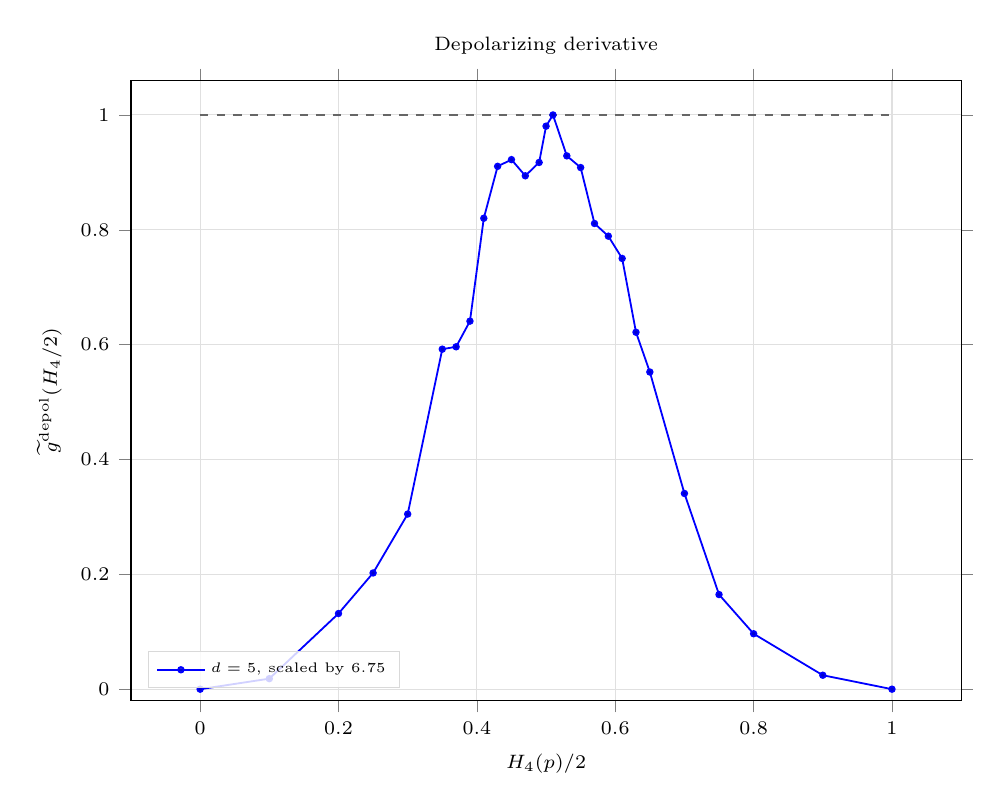
\begin{tikzpicture}
\begin{axis}[
  name=scaledDepolarizingGEXITSurface5Axis,
  width=\linewidth,
  height=0.78\linewidth,
  title={Depolarizing derivative},
  title style={font=\scriptsize},
  xlabel={$H_4(p)/2$},
  ylabel={$\widetilde g^{\rm depol}(H_4/2)$},
  ymin=-0.02, ymax=1.06,
  grid=both,
  major grid style={black!12},
  minor grid style={black!6},
  tick align=outside,
  tick label style={font=\scriptsize},
  label style={font=\scriptsize},
  legend cell align={left},
  legend style={draw=black!15, fill=white, fill opacity=0.82, text opacity=1, at={(0.02,0.02)}, anchor=south west, font=\tiny},
]
\addplot[black!60, dashed, line width=0.55pt, forget plot] coordinates {(0,1) (1,1)};
\addplot+[color=blue, mark=*, mark size=1.0pt, line width=0.65pt]
coordinates {(0,0) (0.1,0.0183355381657) (0.2,0.131766087756) (0.25,0.20239030365) (0.3,0.304956269258) (0.35,0.592128660869) (0.37,0.596263249965) (0.39,0.640933805523) (0.41,0.820139832879) (0.43,0.910519069314) (0.45,0.922195874743) (0.47,0.894025232967) (0.49,0.917300730169) (0.5,0.980480858874) (0.51,1) (0.53,0.928751533852) (0.55,0.908383390125) (0.57,0.810978969476) (0.59,0.788922680475) (0.61,0.750093178513) (0.63,0.621546625027) (0.65,0.552349244688) (0.7,0.340824081702) (0.75,0.164789413162) (0.8,0.0965426550718) (0.9,0.0243044887997) (1,0)};
\addlegendentry{$d=5$, scaled by $6.75$}
\end{axis}
\end{tikzpicture}
